% ==> expandable function: extract last hash str from an outside file
\InputIfFileExists{ztikz-cfg.tex}{}{}
\documentclass{article}
\usepackage[file-io]{ztool}


\begin{document}
\ExplSyntaxOn
% --> write to file
% \seq_set_from_clist:Nn \l_tmpa_seq { {Label-A:111, 222}, {Label-B:333, 444} }
% \ztool_write_seq_to_file:nNn {\c_true_bool} \l_tmpa_seq {Hash.txt}

% --> read from file
% \ztool_read_file_as_seq:nnN {\c_true_bool} {Hash.txt} \l_tmpa_seq
% \seq_show:N \l_tmpa_seq %
% \seq_set_split:NnV \l_tmpb_seq {:} \l_tmpa_seq % ---> not working
% \seq_show:N \l_tmpb_seq %

% --> real wolrd application
% The sequence \l_tmpa_seq contains the items (without outer braces):
% > {sinGraphLabel:3F174D2DE0560706B9CF812E5D220D12,16A7D3AA00F063BC9040C3D92A92A9D0,733AA52DAB26B2961D11D2218473F001}
% > {sinGraphLabel-II:D2A6229667374E17AB5A9634534F18D2}.
\seq_set_from_clist:Nn \l_tmpb_seq { {Label-A=111,222}, {Label-B=333,444} }
% \seq_show:N \l_tmpb_seq 
\prop_set_from_keyval:NN \l_tmpa_prop \l_tmpb_seq
\prop_show:N \l_tmpa_prop
\ExplSyntaxOff

--> BUG of '@' from external file
\ior_open:Ne \g__ztikz_wolfram_ior {\wolframOuputFile}
\ior_get:NN  \g__ztikz_wolfram_ior \l__ztikz_wolfram_tmp_res_tl
\makeatletter
\tl_if_eq:VnTF \l__ztikz_wolfram_tmp_res_tl {@~}
  {\typeout{------>Equal}}
  {\typeout{------>NOT~Equal}}
\typeout{EXPL3----->\the\catcode`\@}
\typeout{FILE----->\exp_after:wN \the\exp_after:wN \catcode\exp_after:wN `\l__ztikz_wolfram_tmp_res_tl}
\end{document}




% ==> new cache mechanism test
\InputIfFileExists{ztikz-cfg.tex}{}{}
\documentclass{article}
\usepackage[library={python, cache, wolfram}]{ztikz}
\usepackage{xcolor}
\usepackage{tabularray}
\usepackage{amsmath}


% \begin{document}
% \sympy{aaa}{1+1}    % ---> works well when 'cache' library not load

% \wolfram{bbb}{1+1}  % ---> works well when 'cache' library not load
% \wolframResult
% \end{document}


% \ztikzHashClean
\ExplSyntaxOn
% ==> token analysis
\seq_new:N \l__token_analysis_seq
\seq_clear:N \l__token_analysis_seq
\cs_set:Npn \__token_analysis:n #1 
  {
    \tl_map_inline:nn {#1}
      {
        \tl_set:Ne \l_tmpa_tl {\number`##1}
        \tl_set:Ne \l_tmpb_tl {\the\catcode`##1}
        \seq_put_right:Ne \l__token_analysis_seq 
          { \exp_not:n {##1}{\l_tmpa_tl : \l_tmpb_tl} } 
      }
    \typeout{------->~~token~analysis~start~<--------}
    \typeout{\seq_use:Nn \l__token_analysis_seq {}}
    \typeout{------->~\space token~analysis~end\space\space<--------^^J}
    \errmessage{Press~ ENTER~ to~ continue}
  }
\cs_set_eq:NN \__tl_debug:n \__token_analysis:n
\cs_generate_variant:Nn \__tl_debug:n { V, e, o }
\cs_generate_variant:Nn \__token_analysis:n { V, e, o }
\NewDocumentCommand{\tokenAnalysis}{m}
  {\__token_analysis:n {#1}}
\ExplSyntaxOff

\begin{document}
% ztikz.hash
% sinGraphLabel:3F174D2DE0560706B9CF812E5D220D12,16A7D3AA00F063BC9040C3D92A92A9D0
% sinGraphLabel-II:D2A6229667374E17AB5A9634534F18D2

\section{python module}
% \ztikzForceToRun
\ztikzForceToSkip
\begin{pyfig}{sinGraphLabel}{sin_graph.pdf}
import matplotlib
matplotlib.use('Agg')
from matplotlib import pyplot as plt
import numpy as np
x = np.linspace(0, 2*np.pi, num = 80)
y = np.sin(x)*np.cos(x)+.2
plt.plot(x, y, 'r-o')
\end{pyfig}
\begin{center}
\includegraphics[width=.5\linewidth]{\pyfigOutputFile}
\end{center}


Hello world:
\ztikzCachedHash[label=sinGraphLabel-II]


\begin{pyfig}{sinGraphLabel-II}{sin_graph.pdf}
import matplotlib
matplotlib.use('Agg')
from matplotlib import pyplot as plt
import numpy as np
x = np.linspace(0, 2*np.pi, num = 80)
y = np.sin(x)*np.cos(x)+.2
plt.plot(x, y, 'b-o')
\end{pyfig}
Hello world:
\ztikzCachedHash[label=sinGraphLabel, index=-2]

\ztikzForceToSkip
% \ztikzForceToRun
1 + 1 = \sympy{aaa}{1+10}


\ztikzForceToSkip
% \ztikzForceToRun
\begin{pycode}{bbb}{pycode_table.txt}
import numpy as np

# write file
with open ('pycode_table.txt', 'w') as file:
  file.write("\\begin{tabular}{p{3cm}ccc}\n")
  file.write("\\hline\n")
  file.write("number/function & $\\sin$ & $\\cos$ & $\\tan$\\\\\n")
  file.write("\\hline\n")
  for i in range(1, 16):
    file.write(
      f"${i}$ & ${np.around(np.sin(i), decimals=4)}$ &  ${np.around(np.cos(i), decimals=4)}$ & ${np.around(np.tan(i), decimals=4)}$\\\\\n"
    )

  file.write("\\hline\n")
  file.write("\\end{tabular}\n")
\end{pycode}
\begin{center}
\input{\pycodeOutputFile}
\end{center}


\section{wolfram module}
% \ztikzForceToRun
% \ztikzForceToSkip
\wolfram*{wolfram-1+1}{1/2}
\[\wolframResult\]

\wolfram{wolframLaplace}{LaplaceTransform[t^4 Sin[3*t], t, s]}
\[
  \mathcal{L}(t^4\sin(3t)) = \wolframResult
\]

\wolframTex{wolframTexInt}{\int_a^b\sin(x)\,dx}
\[
  \int_a^b \sin(x)\,dx = \wolframResult
\]


\wolframTable*{wolframTable}[
  format=cccc, hdbt-rule,
  header={$x$ & $x^2$ & $x^3$ & $x^4$},
  cell-cmd={\textcolor{red}{(#1)}}
]{Table[{i, i^2, i^3, i^4}, {i, 6}]}
\SetTblrOuter{expand=\wolframTableFData}
\hskip6em
\begin{tblr}
  {
    colspec = {cccc}, 
    rowspec = {
      |[2pt,green7]Q|[2pt, teal7]Q|[green7]Q|[green6]
      Q|[green5]Q|[green4]Q|[green3]Q|[3pt,teal7]
    }
  } \wolframTableFData
\end{tblr}


% \ztikzForceToSkip
\wolframSolve{wolframSolve-I}[var={x, y}]{a x + y == 8 && b x - y == 1}
\begin{align}
  &  \wolframResult \\
  &  \wolframResult[||] \\
  &  \wolframResult* \\
  &  \wolframResult*[3-1]
\end{align}
\wolframSolve{wolframSolve-II}
  [var={x, y}, domain=Integers]
  {x^2 + 2 y^3 == 3681 && x > 0 && y > 0}
\begin{align}
  \wolframResult
\end{align}


\wolframDSolve{wolframDSolve-I}{y'[x] + y[x] == a*Sin[x], y[0] == 1}
\begin{align}
  &\wolframResult
\end{align}

% \ztikzForceToSkip
\wolframDSolve{wolframDSolve-II}
  [depend={y[x], z[x]}]
  {y'[x] == Exp[z[x]] + 1, z'[x] == y[x] - x}
\begin{align}\left\{\begin{aligned}
  &\wolframResult[\\&]
\end{aligned}\right.\end{align}


\ztikzForceToSkip
% \ztikzForceToRun
\begin{wolframGraphics}{wolframSinGraph}
  FIGURE=Plot[Sin[x], {x, -Pi, Pi}]hajksdhg
\end{wolframGraphics}

\includegraphics[width=.5\linewidth]{\wolframOuputFile}


\ExplSyntaxOn\makeatletter
\makeatother\ExplSyntaxOff
% \tokenAnalysis{a$@$c#|*}
\end{document}








% ==> stop development sign
\InputIfFileExists{ztikz-cfg.tex}{}{}
\documentclass{../../zlatex/code/ztex}


\title{TEST INTERFACE}
\author{Eureka}
\date{\today}
\begin{document}
\ExplSyntaxOn
\zpagemask[position={(0pt, .25\zph)}, anchor=l]{
  \rlap{\color{gray!25}\rule{\zpw}{6em}}
  \hcoffin_set:Nn \l_tmpa_coffin {\sffamily\Large\color{black!75} For some special rejal ahdj hdah cdhj chjhjahd.}
  \coffin_typeset:Nnnnn \l_tmpa_coffin {hc}{vc}{.5\zpw}{3em}
}
\ExplSyntaxOff
\maketitle

Hello world
\end{document}




% ==> force to run and vice versa test
\InputIfFileExists{ztikz-cfg.tex}{}{}
\documentclass{article}
\usepackage[margin=2.5cm]{geometry}
\usepackage{ztikz}
\ztikzloadlib{cache, python, wolfram}


\begin{document}
% \ztikzForceToRun
% A simple TEST: $1 + 1 = \sympy{1+1}$;


% \ztikzForceToSkip
% A simple TEST II: $1 + 2 = \sympy{1+6}$;


% % \ztikzForceToRun
% \begin{pycode}{anything.pdf}
% import matplotlib
% matplotlib.use('Agg')
% from matplotlib import pyplot as plt
% import numpy as np
% x = np.linspace(0, 2*np.pi, num = 80)
% y = np.sin(x)*np.cos(x)+.2
% plt.plot(x, y, 'r*')
% plt.savefig('anything.pdf')
% \end{pycode}
% \begin{center}
%   \includegraphics[width=.75\linewidth]{\pycodeOutputFile}
% \end{center}


% \ztikzForceToRun
% \ztikzForceToSkip % BUG
% \begin{pycode}{anything.pdf}
% import matplotlib
% matplotlib.use('Agg')
% from matplotlib import pyplot as plt
% import numpy as np
% x = np.linspace(0, 2*np.pi, num = 80)
% y = np.sin(x)*np.cos(x)+.2
% plt.plot(x, y, 'b-o')
% plt.savefig('anything.pdf')
% \end{pycode}
% \begin{center}
%   \includegraphics[width=.75\linewidth]{\pycodeOutputFile}
% \end{center}

% \ztikzForceToRun
\ztikzForceToSkip
\wolfram{1+3} 
% hash of '1+2': 2221D09747385E6860E62CD13C7727F4
1 + 1 = \wolframResult
\end{document}






\documentclass{article}
\begin{document}
% \newcommand{\MyFunction}[1]{#1---#1}
\newcommand{\MyFunction}[1]{(#1)}

\ExplSyntaxOn

\cs_new:Nn \__zpding_ii:n { \MyFunction { #1 } , }
\cs_new:Nn \__zpding_i:n 
  {{ 
    \clist_use:en { \clist_map_function:nN { #1 } \__zpding_ii:n  } 
      { & } 
  },}
\clist_set:Nn \l_tmpa_clist { { a1, a2, a3 } , { b1, b2, b3 } }
\cs_generate_variant:Nn \clist_use:nn { en }
\tl_set:Ne \l_tmpb_tl
  {
    \clist_use:en
      { \clist_map_function:NN \l_tmpa_clist \__zpding_i:n }
      { \\ }
  }
\tl_show:N \l_tmpb_tl % > \l_tmpb_tl=(a1)&(a2)&(a3)\\(b1)&(b2)&(b3).

% \begin{tabular}{ccc}
% \l_tmpb_tl
% \end{tabular}

\ExplSyntaxOff
\end{document}



% wolfram table in tabularray
\InputIfFileExists{ztikz-cfg.tex}{}{}
\documentclass{article}
\usepackage[margin=2.5cm]{geometry}
\usepackage{xcolor, tabularray}
\usepackage[wolfram = { engine=wolfram }]{ztikz}
\ztikzloadlib{cache, wolfram, l3draw}


\begin{document}
% \wolframTable*[
%   format=ccccc, 
%   header={$x$ & $x^2$ & $x^3$ & $x^4$},
%   cell-cmd={\textcolor{red}{(#1)}}
% ]{Table[{i, i^2, i^3, i^4}, {i, 6}]}
\wolframTable*[
  cell-cmd={\textcolor{red}{(#1)}},
  hdbt-rule,
  header={$x$ & $x^2$ & $x^3$ & $x^4$},
]{Table[{i, i^2, i^3, i^4}, {i, 6}]}

\vskip4em
\dotfill\par
(tabular) PART DATA
\begin{tabular}{cccc}
  \wolframTablePData
\end{tabular}

\vskip4em
\dotfill\par
(tabular) FULL DATA
\begin{tabular}{llll}
  \wolframTableFData
\end{tabular}


\ExplSyntaxOn
% \cs_show:N \__wolfram_table_cell_cmd:n
% \show\wolframTablePData
% \show\wolframTablePData
\ExplSyntaxOff
\vskip4em
\dotfill\par
\SetTblrOuter{expand=\wolframTablePData\wolframTableFData}
(tabularray) PART DATA
\begin{tblr}[
    expand+=\expanded,
  ]{
    colspec={cccc}, 
    rowspec={|[2pt,green7]Q|[teal7]Q|[green7]Q|[green6]Q|[green5]Q|[green4]Q|[3pt,teal7]}
  }
  % \wolframTableFData   % --> bug in 'tabularray': cell-cmd lose ??
  \wolframTablePData
\end{tblr}

(tabularray) FULL DATA
\begin{tblr}
  {
    colspec={cccc}, 
    rowspec={|[2pt,green7]Q|[teal7]Q|[green7]Q|[green6]Q|[green5]Q|[green4]Q|[green3]Q|[3pt,teal7]}
  }
  \wolframTableFData   % --> works
\end{tblr}


\zplot[
domain={0, 0.02*3.1415, 2*3.1415},
action=shade, startColor=blue,
endColor=green, axis=x]{sin(x)}
\zplot[
domain={0, 0.02*3.1415, 2*3.1415},
action=shade, startColor=blue,
endColor=green, axis=y]{sin(x)}
\end{document}





\def\totab#1{\totabA#1\relax}
\def\totabA#1{\totabC#1,\relax \cr \totabB}
\def\totabB#1{\ifx,#1\expandafter\totabA\fi}
\def\totabC#1,#2{\ifx\relax#2[#1]\else [#1]&\afterfi{\totabC #2}\fi}
\def\afterfi #1#2\fi{\fi#1}

\message{... \totab{{a1, a2, a3}, {b1, b2, b3, b4}} ...}
\bye



\documentclass{article}
\begin{document}
\ExplSyntaxOn
\clist_set:Nn \l_tmpa_clist {{a1, a2, a3}, {b1, b2, b3}}

\cs_set:Nn \__zpding_one_row:n { \clist_use:nn { #1 } { & } \\ }

\tl_set:Ne \l_tmpb_tl 
  { \clist_map_function:NN \l_tmpa_clist \__zpding_one_row:n }
\tl_show:N \l_tmpb_tl 
\ExplSyntaxOff
\end{document}



\documentclass{article}

\begin{document}
\ExplSyntaxOn
% --> 1 loop
% \cs_set:Npn \_item_cmd:n #1
%   { & (#1) }
% \clist_set:Nn \l_tmpa_clist {a, b, c}
% \tl_set:Ne \l_tmpa_tl 
%   {
%     \clist_map_function:NN \l_tmpa_clist 
%       \_item_cmd:n
%   }
% \cs_generate_variant:Nn \tl_tail:n { e }
% \exp_args:NNe \tl_set:Ne \l_tmpa_tl 
%   { \exp_not:N \tl_tail:n { \l_tmpa_tl } }
% \tl_show:N \l_tmpa_tl % > \l_tmpa_tl=(a)&(b)&(c).


% --> 2 loop
\clist_set:Nn \l_tmpa_clist {{a1, a2, a3}, {b1, b2, b3}}
\cs_set:Npn \__item_cmd:n #1
  { (#1) & }
\cs_set:Npn \__row_cmd:n #1 
  {
    \clist_map_function:nN {#1} 
      \__item_cmd:n \\
  }
\tl_set:Ne \l_tmpb_tl 
  {
    \clist_map_function:NN \l_tmpa_clist 
      \__row_cmd:n
  }
\tl_show:N \l_tmpb_tl % > \l_tmpb_tl=(a1)&(a2)&(a3&\\(b1)&(b2)&(b3&\\.
\ExplSyntaxOff
\end{document}






% implement '\wolframTable' function
\InputIfFileExists{ztikz-cfg.tex}{}{}
\documentclass{article}
\usepackage{xcolor}
\usepackage[wolfram = { engine=wolfram }]{ztikz}
\ztikzloadlib{cache, wolfram}
% \ExplSyntaxOn
% ==> TO PARSER DATA IN FORM: {{x, x ^ 2, x ^ 3}, {1, 1, 1}, {2, 4, 8}, {3, 9, 27}, {4, 16, 64}, {5, 25, 125}}
% \cs_set:Npn \__table_item_handle:n #1 
%   { #1 & }
% \cs_set:Npn \__table_row_handle:n #1
%   { 
%     \clist_map_function:nN { #1\use_none:n }
%       \__table_item_handle:n \\
%   }
% \cs_set:Npn \__typeset_table:nn #1#2 
%   {% #1:table format; #2:table data
%     \begin{tabular}{#1}
%       \hline #2 \hline
%     \end{tabular}
%   }
% % {1, 1, 1, 1}, {2, 4, 8, 16}, {3, 9, 27, 81}
% \cs_new:Npn \part_table_from_file:nN #1#2 
%   {% #1:file ; #2:data var
%     \ztool_gread_file_as_seq:neN {\c_true_bool}
%       { #1 } \l_tmpa_seq
%     \tl_set:Ne #2 { \seq_item:Nn \l_tmpa_seq {1} }
%     \exp_last_unbraced:NNV \tl_set:Ne #2 #2
%     \tl_set:Ne #2
%       {
%         \clist_map_function:oN { #2 } 
%           \__table_row_handle:n
%       }
%   }
% \cs_generate_variant:Nn \clist_map_function:nN { oN }
% \cs_generate_variant:Nn \__typeset_table:nn { ne, no, nV }
% \cs_generate_variant:Nn \part_table_from_file:nN { e, V }
% \tl_new:N \l_part_table_data_tl
% \tl_new:N \l_full_table_data_tl
% \cs_set:Npn \full_part_table_from_file:nnn #1#2#3
%   {% #1:file; #2:table format; #3:table header
%     \part_table_from_file:eN 
%       { #1 } \l_part_table_data_tl
%     \tl_set:Ne \l_full_table_data_tl
%       { 
%         \tl_if_empty:eF {#3}
%           {#3 \\\exp_not:N \hline } 
%         \l_part_table_data_tl 
%       }
%   }
% \NewDocumentCommand{\TableFromFile}{mmm}
%   { 
%     % generate full table data
%     \full_part_table_from_file:nnn {#1}{#2}{#3} 
%     % typeset this table
%     \__typeset_table:no {#2}{\l_full_table_data_tl}
%   }
% \ExplSyntaxOff
% \wolfram*{Table[{i, i^2, i^3, i^4}, {i, 6}]}
% \begin{center}
%   \wolframTable{\wolframOuputFile}{cccc}
%     {$x$ & $x^2$ & $x^3$ & $x^4$ }
% \end{center}



\begin{document}
Hello world \dotfill\par

\vskip3em
\wolframTable*[
  format=ccccc, 
  header={$x$ & $x^2$ & $x^3$ & $x^4$},
  cell-cmd={\textcolor{red}{(#1)}}
]{Table[{i, i^2, i^3, i^4}, {i, 6}]}
% \begin{center}
%   \begin
% \end{center}


% \wolframTable*{Join[{{$x$, $x^2$, $x^3$}}, Table[{i,i^2,i^3}, {i,5}]]} % bug: ''{$x$, $*$x^2, $*$x^3}''

\end{document}






% ==> wolfram cloud / mathics config
\InputIfFileExists{ztikz-cfg.tex}{}{}
\documentclass{article}
\usepackage[
  library={wolfram},
  % wolfram={cloud=false, engine=mathics}
]{ztikz}
% \ztikzloadlib{cache}
\ExplSyntaxOn
\def\curHASH{\tl_use:N \l__ztikz_current_hash_tl}
\ExplSyntaxOff


\begin{document}
Hello world

% \begin{tikzpicture}
% \draw[gray] (-2, -1) grid (2, 2);
% \ShowPoint[color=teal, radius=2pt, type=pentagon*, opacity=.8, rotate=60]
%   {(-1.5, 0); (2, .5)}[$O=(0, 0)$; $(\pi, 0)$]
%   [above right=3pt and 0em, font=\small]
% \end{tikzpicture}

% \wolfram{LaplaceTransform[t^4 Sin[3*t], t, s]}
% \wolfram{101/123 + 124/179}
% \[
%   \mathcal{L}(t^4\sin(3t)) = \wolframResult
% \]

% \begin{wolframGraphics}
%   FIGURE=Plot[Sin[x], {x, -Pi, Pi}]
% \end{wolframGraphics}
% \includegraphics[width=.5\linewidth]{\wolframOuputFile}


% \ztikzHashchgNorun{2E0D5457C90B9A5E88888FCA300716A2}
\wolframTex{\int_a^b2\sin(x)\,dx}
% \ztikzHashCurrent* % CURRENT FILE:'2E0D5457C90B9A5E88888FCA300716A2.wls'
\[
  \int_a^b \sin(x)\,dx = \wolframResult
\]
\end{document}



% ==> expandale token replace command
\documentclass{article}
\usepackage[T1]{fontenc}

\begin{document}
\ExplSyntaxOn
\cs_generate_variant:Nn \tl_map_function:nN { e, V }

\group_begin:
  \char_set_catcode_escape:n { 36 }
  \char_set_catcode_letter:n { 92 }
  $cs_gset:Nn $__double_backslash:n 
    { $tl_if_eq:NNTF #1\ {\\}{#1} }
  $gdef$TEST{
    $char_set_catcode_letter:n { 92 }   % '\'
    $TESTGetARG
  }
  $gdef$TESTGetARG#1{
    $tl_set:Ne $l_tmpa_tl 
      {
        $tl_map_function:nN {#1}                            
          $__double_backslash:n
      }
    $tl_show:N $l_tmpa_tl
    $char_set_catcode_escape:n { 92 }
  }
  $char_set_catcode_escape:n { 92 }
  $char_set_catcode_letter:n { 36 }
\group_end:
\ExplSyntaxOff

Hello world: |\TEST{\abc1\23\def4}| this is an equation below:
$$
  1 + 1 = \alpha + \beta = 2
$$
\end{document}


\documentclass{article}
\usepackage[T1]{fontenc}

\begin{document}
\ExplSyntaxOn
\cs_generate_variant:Nn \tl_map_function:nN { e, V }

\group_begin:
  \char_set_catcode_escape:n { 36 } % '$': escape char
  $char_set_catcode_letter:n { 92 } % '\'
  $cs_gset:Nn $__double_backslash:n 
    { $tl_if_eq:NNTF #1\ {\\}{#1} } % '$'
  $char_set_catcode_escape:n { 92 } % '\': restore escape
  \char_set_catcode_letter:n { 36 } % '$': restore letter
\group_end:

% \tl_set:Nn \l_tmpa_tl {\abc1\23\def}
% \tl_set_rescan:NnV \l_tmpa_tl {\cctab_select:N \c_str_cctab} \l_tmpa_tl
\str_set:Nn \l_tmpa_str {\abc1\23\def}
\group_begin:
  \char_set_catcode_escape:n { 36 }
  \char_set_catcode_letter:n { 92 }
  % $cs_gset:Nn $TEST:n #1
  %   {
  %     $tl_map_function:nN {#1}
  %       $__double_backslash:n
  %   }
  % $cs_generate_variant:Nn $TEST:n { V, e }
  $xdef$TEST#1{
    % $tl_map_function:nN {\abc1\23\def4} 
    % $tl_map_function:nN {$tl_to_str:n {#1}}  % bug
    % $tl_map_function:VN $l_tmpa_tl   % failed
    % $tl_map_function:nN $l_tmpa_str  % failed
    $tl_map_function:eN {#1}         
      $__double_backslash:n
  }
  % $show$TEST
  $char_set_catcode_escape:n { 92 }
\group_end:
% \exp_args:NV \TEST \l_tmpa_str % failed
\char_set_catcode_escape:n { 124 } % '|': escape char
|char_set_catcode_letter:n { 92 } % '\'
|TEST{\abc1\23\def4}
|char_set_catcode_escape:n { 92 }
\ExplSyntaxOff

% \verb|\TEST| is: \TEST{abc}. and Hello world 

% $$\alpha + \beta = \gamma$$
\end{document}




% ==> roboust externalize test
\InputIfFileExists{ztikz-cfg.tex}{}{}
\documentclass{article}
% \usepackage{robust-externalize}
% \cacheEnvironment{tikzpicture}{tikzpicture}
\usepackage{xcolor}
\usepackage{tikz}
\usepackage{xsimverb}
\usepackage{ztool}
\usepackage{xparse}
% \usepackage{ztikz}
% \usetikzlibrary{external}
% \tikzset{external/up to date check={diff}}
% \tikzexternalize[prefix=tikz-cache/]

\makeatletter
\ExplSyntaxOn
% NOT compatible with 'external' library
\tl_new:N \l_ztikz_cache_forward_value_tl
\str_new:N \l_ztikz_cache_forward_name_str
\keys_define:nn {ztikz/cache}
  {
    delimiter  .tl_set:N    = \l_ztikz_cache_arg_delimiter_tl,
    delimiter  .initial:n   = { [] },
    forward    .clist_set:N = \l_ztikz_cache_forward_clist,
    forward    .initial:n   = { \empty },
  }
\cs_new:Npn \__ztikz_cache_deps:n #1 
  {
    \c_percent_str\exp_not:n {#1}:=~#1^^J
  }
\NewDocumentCommand{\ztikzCacheEnv}{om}
  {% #1:new arg-spec; #2:ori-env name; 
  % !! Only single optional arg is permitted
    \DeclareEnvironmentCopy{ztikz@cached@#2}{#2}
    \IfValueT{#1}{ \keys_set:nn {ztikz/cache}{#1} }
    \exp_args:Nne \DeclareDocumentEnvironment{#2}{D\l_ztikz_cache_arg_delimiter_tl{}}
      {% No arg: line content locates at '\begin{<ENV>}' will be gobbled
        % \typeout{--->##1} % --->Mand
        % \typeout{--->##2} % --->HHJKHJKHJ
        % \GetDocumentEnvironmentArgSpec {#2}
        % \typeout{--->\ArgumentSpecification} % --->O{HELLO}mm
        \tl_if_empty:VTF \l_ztikz_cache_arg_delimiter_tl
          { \xsim_file_write_start:nn {\c_true_bool}{ZZZ.tex}\typeout{-->empty~arg} }
          { \xsim_file_write_start:nn {\c_false_bool}{ZZZ.tex} }
      }{
        \xsim_file_write_stop:
        \ztool_insert_to_file:nnn {ZZZ.tex}{1}
          {
            \clist_map_function:NN 
              \l_ztikz_cache_forward_clist 
              \__ztikz_cache_deps:n 
            \exp_not:N\begin{ztikz@cached@#2}
              \tl_item:Nn \l_ztikz_cache_arg_delimiter_tl {1}
              ##1
              \tl_item:Nn \l_ztikz_cache_arg_delimiter_tl {-1}
          }
        \ztool_append_to_file:nn {ZZZ.tex}
          { \exp_not:N \end{ztikz@cached@#2} }
        % \exp_args:No \begin{ztikz@cached@#2}\l_ztikz_cache_arg_delimiter_tl
        % \end{ztikz@cached@#2}
      }
  }
% \ztool_insert_to_file:nnn {temp-w.txt}{3}{NEW-LINE}

% \NewDocumentEnvironment{example}{o}
%   {
%     \IfNoValueTF{#1}
%       {\XSIMfilewritestart*{\jobname-s.txt}}
%       {\XSIMfilewritestart{\jobname-s.txt}}%
%   }{\XSIMfilewritestop}
% \AddToHook{env/ctikzpicture/before}{\begin{example}\begin{ctikzpicture}{Mand}{HHJKHJKHJ}}
% \AddToHook{env/ctikzpicture/after}{\end{example}}
\ExplSyntaxOff
\ztikzCacheEnv[delimiter=[], forward={\AAA,\empty}]{tikzpicture}


\begin{document}
\def\AAA{AAA-aba}

BBB \AAA{} bbb.

% I am a cached picture: \begin{tikzpicture}<forward=\AAA>
% \node[draw,rounded corners,fill=teal!50](A){BBB \AAA{} bbb.};
% \end{tikzpicture}.

% \begin{tikzpicture}
%   \node[draw,rounded corners,fill=teal!50](A){BBB \AAA{} bbb.};
% \end{tikzpicture}

% \pdfmdfivesum file {XXX.tex}
% AAA-aaa. 8CFC240350E96BB198E39BF0C450A522
% AAA-aba. 1425867299391550907B35C5C8C66BD8
% comment check 1: 3CA4F9C40B4A161FDB92DA4E0FD7B89C
% comment check 2: D0B16CF7620A6B4EF806FB3C8228C55B

% \begin{tikzpicture}
%   \node[draw,rounded corners,fill=teal!50](A){BBB \AAA{} bbb.};
% \end{tikzpicture}

\def\BBB{BBB-bbb}
% \begin{example}
% \begin{ctikzpicture}{Mand}{HHJKHJKHJ}
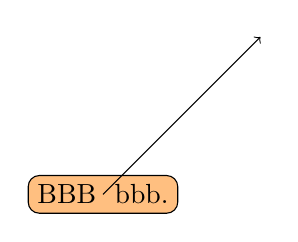
\begin{tikzpicture}[scale=2]
  \node[draw,rounded corners,fill=orange!50](A){BBB \AAA{} bbb.};
  \draw[->] (0, 0) -- (1, 1)node {\BBB};
\end{tikzpicture}
% \end{example}

% \ShowDocumentEnvironmentArgSpec {tikzpicture}
% \typeout{--->\ArgumentSpecification} % --->mm

%\AAA := AAA-aba
%\empty :=
\begin {ztikz@cached@tikzpicture}[scale=2]

  \node[draw,rounded corners,fill=orange!50](A){BBB \AAA{} bbb.};
  \draw[->] (0, 0) -- (1, 1)node {\BBB};
\end {ztikz@cached@tikzpicture}



% --> extract preable on the fly
% \ExplSyntaxOn
% \ztool_gread_file_as_seq:nnN {\c_true_bool}{debug.tex}{\l_tmpa_seq}
% % \seq_show:N \l_tmpa_seq
% \prg_generate_conditional_variant:Nnn \str_if_eq:nn { ne } { TF }
% \prg_generate_conditional_variant:Nnn \str_if_empty:n { e } { F }
% \str_set:Nn \l_tmpa_str {\begin{document}}
% \iow_open:Nn \g_ztool_file_append_iow {extract-preamble.tex}
% \seq_map_inline:Nn \l_tmpa_seq 
%   {
%     \str_if_eq:neTF {#1}{\l_tmpa_str}
%       { 
%         \seq_map_break: 
%         \iow_close:N \g_ztool_file_append_iow
%       }
%       % { \seq_put_right:Nn \l_tmpb_seq {#1} }
%       { 
%         \str_if_empty:eF {\tl_trim_spaces:n {#1}}{
%         \iow_now:Ne \g_ztool_file_append_iow 
%           { \exp_not:n {#1}}
%         }
%       }
%   }
% % \seq_show:N \l_tmpb_seq
% \ExplSyntaxOff
\end{document}




% ===> ApTeX Test
% NOTE:
% 1.'dvipdfm' and 'dvipdfmx' can get graphics dimension
% 2.'dvpdfm' do NOT support fadings
% 3.NOT compatiable with tikz 'external' library
% REF: https://tex.stackexchange.com/a/17737/294585
\InputIfFileExists{ztikz-cfg.tex}{}{}
\documentclass{article}
\def\pgfsysdriver{pgfsys-dvipdfmx.def}
\usepackage[dvipdfmx]{graphicx}
\usepackage{ztikz}
\ztikzloadlibrary{gnuplot, zdraw}


\begin{document}
\section{Normal picture}
\begin{figure}[!htb]
  \centering
  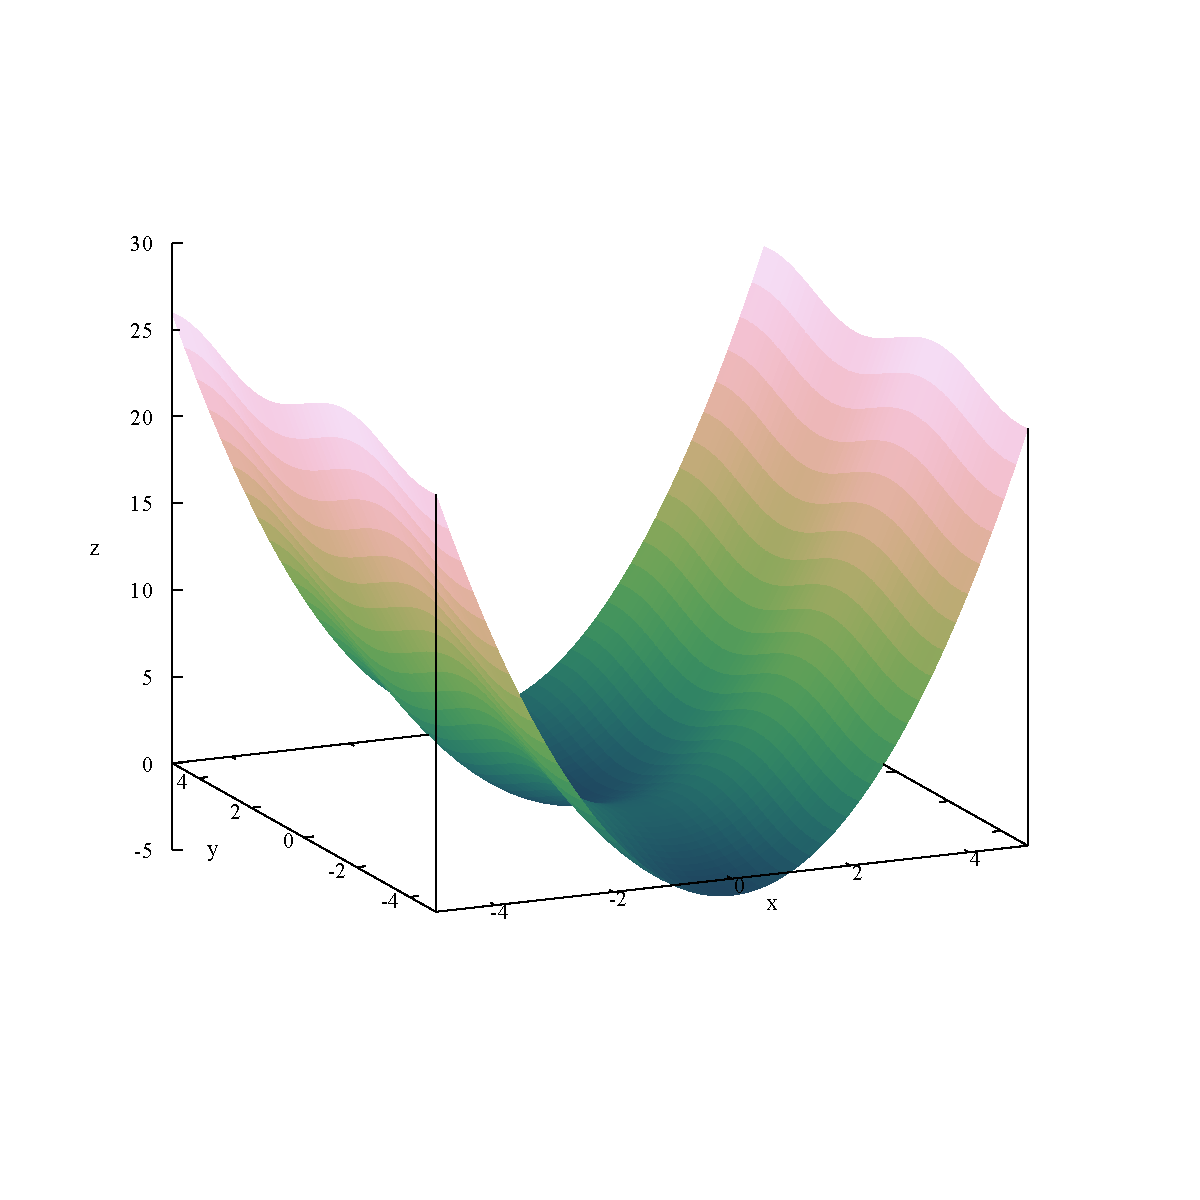
\includegraphics[width=.75\linewidth]{./pics/plot_3d_1.pdf}
  \caption{AAA}
  \label{fig:AAA}
\end{figure}

\section{tikz}
\subsection{builtin}
\begin{tikzpicture}
  \draw[very thin,color=gray] (-0.1,-1.1) grid (3.9,3.9);
  \draw[->] (-0.2,0) -- (4.2,0) node[right] {$x$};
  \draw[->] (0,-1.2) -- (0,4.2) node[above] {$f(x)$};
  \draw[color=red] plot (\x,\x) node[right] {$f(x) =x$};
  % \x r means to convert '\x' from degrees to _r_adians:
  \draw[color=blue] plot (\x,{sin(\x r)}) node[right] {$f(x) = \sin x$};
  \draw[color=orange] plot (\x,{0.05*exp(\x)}) node[right] {$f(x) = \frac{1}{20} \mathrm e^x$};
\end{tikzpicture}


\subsection{ztikz}
\begin{tikzpicture}
\ShowGrid{(-5, -5);(5, 5)}
\Plot[
  domain=0:2*pi, 
  style={color=teal}, 
  marker={type=square*, color=red, rotate=45}
]{2*sin(x)}
\ContourPlot[
  domain={-1.5:1.5;}, 
  style={color=red}, 
]{x**2/4+y**2-1}
\PlotPrecise{param}{100}
\ParamPlot[domain=-pi:pi, style={teal, very thick}]{4*sin(t), 2*cos(t)}
\PolarPlot{2*(1-sin(t))}
\end{tikzpicture}

\subsection{gnuplot}
\Plotz[palette={cubehelix start 0 cycles -1. saturation 1}]{x**2-sin(y)}


\section{l3draw Test}
NOT SUPPORT YET

% \begin{center}
%   \zrule[width=10, startColor=red, step=0.5]
% \end{center}

% \ExplSyntaxOn
% \cs_set_eq:NN \moveto:n \draw_path_moveto:n
% \cs_set_eq:NN \gdraw:n  \draw_path_use_clear:n
% \draw_begin:
%   \int_step_inline:nnnn {0}{45}{360}{
%     \draw_path_circle:nn {
%       \draw_point_polar:nn {2em}{#1}
%     }{2pt}
%   }
%   \gdraw:n {fill}
% \draw_end:
% \ExplSyntaxOff
\end{document}


% ==> hash char catcode
\InputIfFileExists{ztikz-cfg.tex}{}{}
\documentclass{article}
\usepackage{ztool}



\begin{document}
\ExplSyntaxOn
\group_begin:
\char_set_catcode_other:N \#
% \char_set_catcode_other:n { 35 }

% \tl_set_eq:NN \l_tmpa_tl \c_hash_str
\gdef\hashchar{#}
\group_end:

% \ztool_append_to_file:nn {temp-w.txt}
%   {\exp_not:n {#}}

\tl_set:Nn \l_tmpa_tl {\exp_not:n {#1}}
\tl_show:N \l_tmpa_tl
\ExplSyntaxOff


Hello world: \hashchar{} HAHA
\end{document}





% ===> test gif insert
\documentclass{article}
\usepackage{graphicx}
\usepackage{animate}


\begin{document}
\begin{center}
  \animategraphics[
    loop,controls,
    width=.75\linewidth
  ]{10}{./pics/gif/test-gif-converted-to-}{0}{}
\end{center}
\end{document}



\documentclass{article}
\usepackage{graphicx}
\usepackage{epstopdf}
% \epstopdfDeclareGraphicsRule
%   {.gif}{png}{.png}{convert gif:test.gif png:TEST}
\DeclareGraphicsRule{.gif}{png}{.png}{`convert #1 `basename #1 .gif`-gif-converted-to.png}
\AppendGraphicsExtensions{.gif}


\begin{document}
Hello world.

\begin{figure}[!htb]
  \centering
  
\includegraphics[width=.75\linewidth]{test.gif}
  \caption{}
  \label{fig:}
\end{figure}

\end{document}





% ==> test sed replacement
\InputIfFileExists{ztikz-cfg.tex}{}{}
\documentclass{article}
\usepackage{ztikz}
\ztikzloadlibrary{cache, gnuplot}


\begin{document}
\begin{tikzpicture}
\ShowGrid{(-5, -5);(5, 5)}
\Plot[
  domain=0:2*pi, 
  style={color=teal}, 
  marker={type=square*, color=red, rotate=45}
]{2*sin(x)}

\ContourPlot[
  domain={-1.5:1.5;}, 
  style={color=red}, 
]{x**2/4+y**2-1}
\PlotPrecise{param}{6}
\ParamPlot[domain=-pi:pi, style={teal, very thick}]{4*sin(t), 2*cos(t)}
\PolarPlot{2*(1-sin(t))}
\end{tikzpicture}

\Plotz[palette={cubehelix start 0 cycles -1. saturation 1}]{x**2-sin(y)}
\end{document}


% ==> test
\InputIfFileExists{ztikz-cfg.tex}{}{}
\documentclass{article}
\usepackage{graphicx}
\usepackage{amsmath}
\usepackage{ztikz}
\ztikzloadlibrary{cache, python, wolfram}
% \ztikzloadlibrary{wolfram}


\begin{document}
% \ExplSyntaxOn
% \ztool_append_to_file:nn {temp.txt}{XXX-1}

% \ztool_append_to_file:nn {temp.txt}{XXX-2}
% \ExplSyntaxOff

% \begin{pyfig}[width=.45\linewidth]{pycode.py}
% import matplotlib
% matplotlib.use('Agg')
% from matplotlib import pyplot as plt
% plt.rcParams['font.sans-serif'] = ['FangSong']
% plt.rcParams['axes.unicode_minus'] = False
% import numpy as np
% x = np.linspace(0, 2*np.pi, num = 80)
% y = np.sin(x)*np.cos(x)+.2
% plt.plot(x, y, 'ro')
% \end{pyfig}

% \[
%   2^{64} = \py{2**64}
% \]
\begin{wolframGraphics}
FIGURE=Plot[Sin[x], {x, -Pi, Pi}]
\end{wolframGraphics}

\begin{figure}[!htb]
  \centering
  \includegraphics[width=.75\linewidth]{\wolframOuputFile}
  \caption{Wolfram-Ouput-FIGURE}
  \label{fig:Wolfram-Ouput-FIGURE}
\end{figure}

\begin{wolframGraphics}[width=.5\linewidth]
  FIGURE=Plot[Sin[x], {x, -Pi, Pi}]
\end{wolframGraphics}

\wolfram{LaplaceTransform[t^4 Sin[3*t], t, s]}
\[
  \wolframResult
\]

\wolfram{2+2}
\[
  \wolframResult
\]

\wolframSolve[var={x, y}]{a x + y == 8 && b x - y == 1}
\begin{align}
  &  \wolframResult \\
  &  \wolframResult[||] \\
  &  \wolframResult* \\
  &  \wolframResult*[3-1]\\
  &  \wolframResult*[-1] \\
  &  \wolframResult*[a]
\end{align}

\wolframSolve[var={x, y}, domain=Integers]{x^2 + 2 y^3 == 3681 && x > 0 && y > 0}
\begin{align}
  \wolframResult
\end{align}


\wolframSolve[var={x, y}, domain=Integers]{x+y == 5 && x > 0 && y > 0}
\begin{align}
  &\wolframResult[\\&]
\end{align}


\wolframDSolve{y'[x] + y[x] == a*Sin[x], y[0] == 1}
\begin{align}
  &\wolframResult
\end{align}

\wolframDSolve[depend={y[x], z[x]}]{y'[x] == Exp[z[x]] + 1, z'[x] == y[x] - x}
\begin{align}
  &\wolframResult[\\&]
\end{align}
\end{document}


% ==> append to file
\InputIfFileExists{ztikz-cfg.tex}{}{}
\documentclass{article}
\usepackage{../../ztool/code/ztool}


\begin{document}
\ExplSyntaxOn
\ior_new:N \g_file_append_ior
\iow_new:N \g_file_append_iow
\str_new:N \l_file_content_str
\str_clear:N \l_file_ori_content_str
\cs_new:Npn \c_hash_symbol   {\iow_char:N \# }
\cs_new:Npn \c_space_symbol  {\iow_char:N \  }
\cs_new_protected:Npn \__append_to_file:nn #1#2 
  {% #1: file name; #2: content
    \ior_open:Nn \g_file_append_ior {#1}
    \ior_str_map_inline:Nn \g_file_append_ior
      {
        \str_put_right:Nx \l_file_ori_content_str {^^J\tl_to_str:n {##1}}
      }
    \iow_open:Nn \g_file_append_iow {#1}
    \str_remove_once:Nn \l_file_ori_content_str {^^J}
    \iow_now:Ne \g_file_append_iow {\l_file_ori_content_str} 
    \tl_set:Nn \l_tmpa_tl {#2}
    \tl_set_rescan:Nnn \l_tmpa_tl 
      {
        % \cctab_select:N \c_str_cctab
        \char_set_catcode_letter:n {35}
        \char_set_catcode_letter:n {36}
        \char_set_catcode_letter:n {64}
        % \char_set_catcode_letter:n {92}
        \char_set_catcode_letter:n {94}
        \char_set_catcode_letter:n {95}
        % \char_set_catcode_other:N \exp_not:N \~
      }{#2}
    \iow_now:Ne \g_file_append_iow {\l_tmpa_tl}
    \iow_close:N \g_file_append_iow
  }

% \newcommand{\test}{\c_hash_str/$<~ \c_backslash_str@2_#^1>\c_backslash_str *$\c_hash_str|}
\__append_to_file:nn {temp.txt}{ABCD~ EFG}
  
% \ztool_append_to_file:nn {temp.txt}
%   {\c_hash_str/$<~ \c_backslash_str@2_#^1>\c_backslash_str *$\c_hash_str|}
\ExplSyntaxOff

HELLO
\end{document}




\InputIfFileExists{ztikz-cfg.tex}{}{}
\documentclass{article}
\usepackage{ztikz}
\usepackage{xsimverb}
\ztikzloadlibrary{gnuplot}
\ExplSyntaxOn
\newcommand{\xsimStart}[1]{
  \xsim_file_write_start:nn {\c_true_bool}{#1}
}
\newcommand{\xsimEnd}{\xsim_file_write_stop:}

\newenvironment{export}[1]{
  \xsim_file_write_start:nn {\c_false_bool}{#1}
  \gdef\filename{#1}
}{
  \xsim_file_write_stop:
  \expandafter\input\expandafter{\filename}
}
\ExplSyntaxOff
% \AddToHook{env/tikzpicture/before}{\begin{export}{XXX.tex}}
% \AddToHook{env/tikzpicture/after}{\end{export}}


\begin{document}
\section{gnuPlot}
\PlotPrecise{plot}{50}


\def\AAA{aaa}
% \begin{export}{export-2.tex}
\begin{tikzpicture}
  \Plot[
    domain=0:2*pi, 
    style={color=teal}, 
    % marker={type=square*, color=red, rotate=45}
  ]{2*sin(x)}
  \StemPlot[x][red][type=*, color=orange]{\gnudata{1}}
  \node at (0, 0) {\AAA};
\end{tikzpicture}
% \end{export}

% \show\tikzpicture
\end{document}